\normalfalse \difficiletrue \tdifficilefalse
\correctionfalse

%\UPSTIidClasse{11} % 11 sup, 12 spé
%\newcommand{\UPSTIidClasse}{12}

\exer{Résistance équivalente$\star$ \label{C1:06:537}}

\setcounter{question}{0}\marginnote{\xpComp{ELEC}{01}}%\UPSTIcompetence[2]{C1-06}
\index{Compétence C1-06}\index{Compétence ELEC-01}
\index{Grandeurs électriques}
\index{Lois de Kirchhoff}
\ifcorrection
\else
\marginnote{\textbf{Pas de corrigé pour cet exercice.}}
\fi



\question{Déterminer la résistance équivalente du dipole suivant.}
\begin{marginfigure}
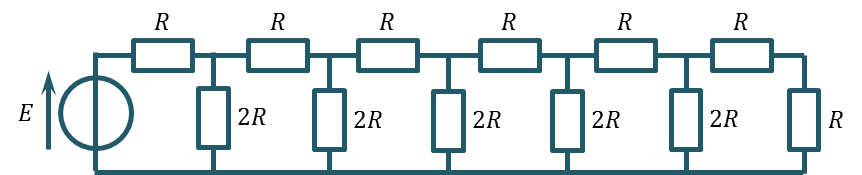
\includegraphics[width=\linewidth]{537_01}
\end{marginfigure}




\ifprof
\else

\marginnote{Corrigé voir \ref{C1:06:537}.}

\fi